\documentclass{beamer}
\usepackage{minted}
\usemintedstyle{default}


\begin{document}

\begin{frame}
\frametitle{Performance Optimisation}
\begin{itemize}
\item The algorithm must be executed for each pixel.
\item For example: $1920 \times 1080 = 2073600$ pixels.
\item Parallel computing allows simultaneous program execution.
\item Multi-threading allows use of multiple CPU cores. On average CPU has 2-8 cores.
\end{itemize}
\end{frame}


\begin{frame}
\frametitle{The Graphics Processing Unit}
\begin{itemize}
\item Designed primarily for computer graphics.
\item Video games, computer aided design (CAD) machine learning.
\item GPUs have 1,000s - 10,000s of cores.
\item Graphics APIs such as OpenGL, Vulkan, Direct3D, Metal.
\item "Shaders" are programs that execute on the GPU.
\item OpenGL has bindings for many languages including Python (via PyOpenGL).
\item Used in conjunction with GUI library (GLUT, Tkinter via pyopengltk)
\end{itemize}
\end{frame}


\begin{frame}
\frametitle{OpenGL Rendering Pipeline}
\begin{columns}
    \begin{column}{0.5\textwidth}
      \begin{itemize}
        \item Programmer specifies vertices.
        \item Specify primitive type (point, line, triangle etc).
        \item Vertex shader program processes them.
        \item Rasterizer breaks down Primatives into Fragments.
        \item Fragment shader colours each pixel individually.
      \end{itemize}
    \end{column}
    \begin{column}{0.5\textwidth}
      \centering
      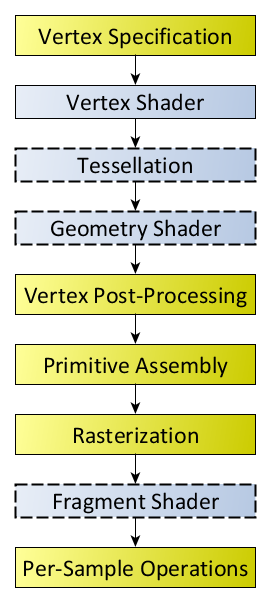
\includegraphics[width=0.6\textwidth]{RenderingPipeline.png}
      \par \tiny {Source: https://www.khronos.org/opengl/wiki\\/Rendering\_Pipeline\_Overview}
    \end{column}
  \end{columns}
\end{frame}


\begin{frame}[fragile]
\frametitle{Fragment Shader}

\begin{minted}[fontsize=\tiny]{glsl}
#version 330 core
uniform vec2 resolution;

out vec4 color;

vec2 f(vec2 c, vec2 z)
{
    return vec2(z.x*z.x - z.y*z.y, 2.0*z.x*z.y) + c;
}

void main()
{
    vec2 z = vec2(0.0, 0.0);
    vec2 coord = (((gl_FragCoord.xy - resolution.xy/2)/resolution.x) * 2.0);
    vec2 c = coord / 0.5;

    int max_iter = 128;
    int i = 0;
    while (i < max_iter && length(z) < 2.0)
    {
        z = f(c, z);
        ++i;
    }

    if (i == max_iter)
    {
        color = vec4(0.0, 0.0, 0.0, 1.0);
    } else {
        color = vec4(1.0, 1.0, 1.0, 1.0);
    }
}

\end{minted}

\end{frame}


\begin{frame}
\frametitle{Fragment Shader}
\centering

\includegraphics[width=1.0\textwidth]{GreyscaleMandelbrot.png}
\end{frame}

\begin{frame}[fragile]
\frametitle{Adding Colour}

\begin{minted}[fontsize=\tiny]{glsl}
#version 330 core
uniform vec2 resolution;

out vec4 color;

vec2 f(vec2 c, vec2 z)

vec3 HSV_to_RGB(vec3 col) {
    vec4 K = vec4(1.0, 2.0 / 3.0, 1.0 / 3.0, 3.0);
    vec3 p = abs(fract(col.xxx + K.xyz) * 6.0 - K.www);
    return col.z * mix(K.xxx, clamp(p - K.xxx, 0.0, 1.0), col.y);
}

void main()
{
    vec2 z = vec2(0.0, 0.0);
    vec2 coord = (((gl_FragCoord.xy - resolution.xy/2)/resolution.x) * 2.0);
    vec2 c = coord / 0.5;

    int max_iter = 128;
    int i = 0;
    while (i < max_iter && length(z) < 2.0)
    {
        z = f(c, z);
        ++i;
    }

    if (i == max_iter)
    {
        color = vec4(0.0, 0.0, 0.0, 1.0);
    } else {
        float t = float(i) / float(max_iter);
        color = vec4(HSV_to_RGB(vec3(t+0.6f, 1.0, 1.0)), 1.0);
    }
}

\end{minted}
\end{frame}


\begin{frame}
\frametitle{Adding Colour}

\includegraphics[width=1.0\textwidth]{ColourMandelbrot.png}
\end{frame}



\begin{frame}[fragile]
\frametitle{Adding Dynamic Visualisation}

\begin{minted}[fontsize=\tiny]{glsl}
#version 330 core
uniform vec2 resolution;
uniform vec2 L_pan;
uniform float scale;

out vec4 color;

vec2 f(vec2 c, vec2 z)
vec3 HSV_to_RGB(vec3 col)

void main()
{
    vec2 z = vec2(0.0, 0.0);
    vec2 coord = (((gl_FragCoord.xy - resolution.xy/2)/resolution.x) * 2.0);
    vec2 c = coord / scale + L_pan;

    int max_iter = 128;
    int i = 0;
    while (i < max_iter && length(z) < 2.0)
    {
        z = f(c, z);
        ++i;
    }

    if (i == max_iter)
    {
        color = vec4(0.0, 0.0, 0.0, 1.0);
    } else {
        float t = float(i) / float(max_iter);
        color = vec4(HSV_to_RGB(vec3(t+0.6f, 1.0, 1.0)), 1.0);
    }
}


\end{minted}
\end{frame}


\begin{frame}
\frametitle{Adding Dynamic Visualisation}

\includegraphics[width=1.0\textwidth]{ZoomedMandelbrot.png}
\par \tiny {Location: $0.78 + 0.13i$}
\end{frame}


\begin{frame}[fragile]
\frametitle{Modules}

\begin{minted}{python}
from OpenGL import GL
import OpenGL.GL.shaders
from pyopengltk import OpenGLFrame
import tkinter as tk
import numpy as np
import ctypes
\end{minted}
\end{frame}

\begin{frame}[fragile]
\frametitle{Shader Compilation}
\begin{minted}[fontsize=\tiny]{python}
# Avoiding glitches in pyopengl-3.0.x and python3.4
def bytestr(s):
    return s.encode("utf-8") + b"\000"


# Avoiding glitches in pyopengl-3.0.x and python3.4
def compileShader(source, shaderType):
    """
    Compile shader source of given type
        source -- GLSL source-code for the shader
    shaderType -- GLenum GL_VERTEX_SHADER, GL_FRAGMENT_SHADER, etc,
        returns GLuint compiled shader reference
    raises RuntimeError when a compilation failure occurs
    """
    if isinstance(source, str):
        source = [source]
    elif isinstance(source, bytes):
        source = [source.decode('utf-8')]

    shader = GL.glCreateShader(shaderType)
    GL.glShaderSource(shader, source)
    GL.glCompileShader(shader)
    result = GL.glGetShaderiv(shader, GL.GL_COMPILE_STATUS)
    if not(result):
        # TODO: this will be wrong if the user has
        # disabled traditional unpacking array support.
        raise RuntimeError(
            """Shader compile failure (%s): %s""" % (
                result,
                GL.glGetShaderInfoLog(shader),
            ),
            source,
            shaderType,
        )
    return shader
\end{minted}
\end{frame}

\end{document}
